\documentclass[12pt, a4paper]{article}
\usepackage{caption}
\usepackage{graphicx}
\usepackage{hyperref}
\hypersetup{
    colorlinks,
    citecolor=black,
    filecolor=black,
    linkcolor=black,
    urlcolor=black
}
\usepackage{tikz-network}
\usepackage{amsmath, amsfonts, amssymb, amsthm}
\usepackage{algpseudocode}
\usepackage{algorithm}
\title{Network and Cybersecurity\\ Exercises}
\date{2022}
\author{Kristoffer Klokker}

\usepackage{xcolor,listings}
\usepackage{textcomp}
\usepackage{color}
\usepackage{listings}
\definecolor{codegreen}{rgb}{0,0.6,0}
\definecolor{codegray}{rgb}{0.5,0.5,0.5}
\definecolor{codepurple}{HTML}{C42043}
\definecolor{backcolour}{HTML}{F2F2F2}
\definecolor{bookColor}{cmyk}{0,0,0,0.90}  
\color{bookColor}

\lstset{upquote=true}

\lstdefinestyle{mystyle}{
    backgroundcolor=\color{backcolour},   
    commentstyle=\color{codegreen},
    keywordstyle=\color{codepurple},
    numberstyle=\numberstyle,
    stringstyle=\color{codepurple},
    basicstyle=\footnotesize\ttfamily,
    breakatwhitespace=false,
    breaklines=true,
    captionpos=b,
    keepspaces=true,
    numbers=left,
    numbersep=10pt,
    showspaces=false,
    showstringspaces=false,
    showtabs=false,
    tabsize=3,
}
\lstset{style=mystyle}
\usepackage{zref-base}


\setcounter{tocdepth}{1}
\makeatletter
\newcounter{mylstlisting}
\newcounter{mylstlines}
\lst@AddToHook{PreSet}{%
  \stepcounter{mylstlisting}%
  \ifnum\mylstlines=1\relax
    \lstset{numbers=none}
  \else
    \lstset{numbers=left}
  \fi
  \setcounter{mylstlines}{0}%
}
\lst@AddToHook{EveryPar}{%
  \stepcounter{mylstlines}%
}
\lst@AddToHook{ExitVars}{%
  \begingroup
    \zref@wrapper@immediate{%
      \zref@setcurrent{default}{\the\value{mylstlines}}%
      \zref@labelbyprops{mylstlines\the\value{mylstlisting}}{default}%
    }%
  \endgroup
}

% \mylstlines print number of lines inside listing caption
\newcommand*{\mylstlines}{%
  \zref@extractdefault{mylstlines\the\value{mylstlisting}}{default}{0}%
}
\makeatother


\newcommand\numberstyle[1]{%
    \footnotesize
    \color{codegray}%
    \ttfamily
    \ifnum#1<10 0\fi#1 |%
}


\begin{document}
	\maketitle
	\clearpage
	\tableofcontents
	\clearpage
	\section{Lecture 1}
		\subsection{Generalize a formula for sending P such packets back-to-back over the N link}
			For a single package the sending time will be:
			$$d_{end-to-end}=N\frac{L}{R}$$
			For a number of packages $P$ the formular wil lbe:
			$$d_{end-to-end}=(P+N)\frac{L}{R}$$
		\subsection{Consider the circuit-switched network in this figure}
			\begin{figure}[h!]
				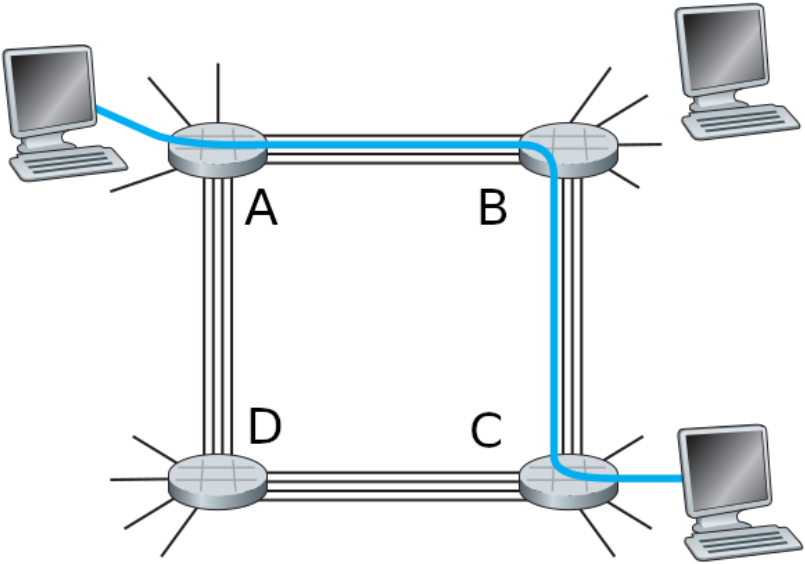
\includegraphics[width=300px]{assets/1.1.png}
				\center
			\end{figure}
			\subsubsection{What is the maximum number of simultaneous conections that can be in progress at the same time in this network}
				Assuming each host can have 4 ingoing and 4 outgoing connections the total number of active connections would be 12. This is where 4 simultaneous connections between the neightboor host.\\
				In case each computer can maximux have 4 ingoing or outgoing connections the total connections would be halfed to 6.
			\subsubsection{Suppose that all connections are between switches A and C. What is the maximum number of simultaneous conections that can be in progress}
				There can only be 4 connections between A and C.
			\subsubsection{Suppose we want to make four connections between switches A and C, and another four connections between B and D. Can we route these calls through the four links to accomodate all eight connections}
				To make a connection one pair can have the two outer links and the other pair can have the two inner links, resulting in 4 links between the pairs.
		\subsection{This elementary problem begins to explore propagation delay and transmission delay, two central concepts in data networking. Consider two hosts, A and B, connected by a single link of rate R bps. Suppose that the two hosts are separated by $m$ meters, and suppose the propagation speed along the link is $s$ meters/sec. Host A is to send a packet of size $L$ bits to Host B}
			\subsubsection{Express the propagation delay, $d_{prop}$ in terms of $m$ and s.}
				
				$$d_{prop} = \frac{m}{s}$$
			\subsubsection{Determine the transmission time of the packet $d_{trans}$ in terms of $L$ and $R$}
				$$d_{trans}=\frac{L}{R}$$
			\subsubsection{ Ignoring processing and queuing delays, obtain an expression for the end-to-end delay}
				$$d_{trans}+d_{prop}=\frac{m}{s}\cdot \frac{L}{R}$$
			\subsubsection{Suppose Host A begins to transmit the packet at time $t=0$. At time $t=d_{trans}$ where is the last of the packet}
				It would be in the link, since it would then have gathered the entire package
			\subsubsection{Suppose $d_{prop}$ is greater than $d_{trans}$. At time $t=d_{trans}$ where si the first bit of the packet.}
				It would be in the link, since the link have to gather the entire package before sending it off
			\subsubsection{Suppose $s=2.5\cdot 10^8$, $L=120$bits and $R=56$kbps. Find the distance $m$ so that $d_{prop}=d_{trans}$}
				\begin{align*}
					d_{trans}=\frac{L}{R}=\frac{120}{56000}=0.00214\\
					d_{prop}=\frac{m}{s}=\frac{m}{2.5\cdot 10^8}=d_{trans}\\
					m=d_{trans}\cdot 2.5\cdot 10^8=535.714
				\end{align*}
				Assuming that $s$ is in the unit meters/sec the distance would be 535.714 meters
		\subsection{Suppose N packets arrive simultaneously to a link at which no packets are currently being transmitted or queued. Each packet is of length L and the link has transmission rate R.}
			\subsubsection{What is the average queing delay for the $n$ packets}
				$$\frac{L\cdot P/2}{R}$$
				On average the packet would be in the middle of queue and therefore be half of $P$
			\subsubsection{Now suppose that N such packets arrive to the link every LN/R seconds. What is the average queuing delay of a packet?}
				Since the package arrival is faster than the package handling time, in the case of an infinite size buffer the aver delay would be infinite
		\subsection{Suppose two hosts A and B are speareated by 20,000 kilometers and are conencted by a direct link of R=2 Mbs. Suppose the propagation speed of the link is $s=2.5\cdot 10^8$ meters/sec}
			\subsubsection{Calculate the bandwidth-delay product $R\cdot d_{prop}$}
				$$R\cdot \frac{m}{s}=2\cdot 10^6b/s\cdot \frac{20,000,000m}{2.5\cdot 10^8m/s}=160Kb$$
			\subsubsection{Consider sending a file of 800,000 bits from Host A to Host B. Suppose the file is sent continuously as one large message. What is the maximum number of bits that will be in the link at any given time}
				160Kb as found in last exercise
			\subsubsection{Provide an interpretation of the bandwidth-delay product}
				Bandwidth-delay product is the number if bits which can exist in the link at one time every second.
			\subsubsection{What is the width of a bit in the link}
				$$\frac{20,000,000m}{160,000b}=125m$$
			\subsubsection{Derive a general expression for the width of a bit in terms of the prpagation speed $s$, the transmission rate $R$ and the length of the link $m$.}
				$$\frac{m}{R\cdot \frac{m}{s}}=\frac{s}{R}$$
		\subsection{Suppose there is a 10 Mbps microwave link between a geostationary satellite and its base station on Earth. Every minut the satellite takes a digital photo and sends it to the base station. Assume a propagation speed of $s=2.5\cdot 10^8$ meters/sec.}
			\subsubsection{What is the propagation delay of the link}
				$$\frac{m}{s}= \frac{35,786,000m}{2.5\cdot 10^8m/s}= 0.143s$$
			\subsubsection{What is the bandwidth delay product of the link}
				$$R\cdot \frac{m}{s}=10^7b\cdot \frac{35,786,000m}{2.5\cdot 10^8m/s}=1.43Mb$$
			\subsubsection{Let x denote the size of the photo. What is the minimum value of x for the microwave link the be contrinously transmitting}
				There are 86400 seconds in a day, therefore the minumum size of the photo would be:
				$$1.43Mb/s \cdot 86400s = 123.5Gb$$
		\subsection{Would it be faster to ship 300 terabytes over night than transfer with 1 Gbps}
			$$\frac{300,000Gb}{1Gb/s}=300,000s= 83.33 hours$$
			it would therefore be faster to ship the harddrive
	\section{Lecture 2}
		\subsection{Assume you request a webpage consisting of one document and five images. The document size is 1 kbyte, all images have the same size of 50 kbytes, the download rate i 1 Mbps, and the RTT is 100 ms. How long does it take to obtain the whole webpage under the following conditions? }
			\begin{itemize}
				\item Nonpersistent HTTP with serial connection - 
				\begin{align*}
					= 6 \cdot 2\cdot 100ms + (1kbyte + (5\cdot 50)kbytes)/1Mbps\\
					=1200ms + (8kb + 2000kb)/1000kbps\\
					=1200ms + 2008ms\\
					=3208ms
				\end{align*}
				\item Nonpersistent HTTP with two parrallel connections - 
				\begin{align*}
					= 6 \cdot 2\cdot 100ms / 2 + (1kbyte + (5\cdot 50)kbytes)/1Mbps\\
					=600ms + (8kb + 2000kb)/1000kbps\\
					=600ms + 2008ms\\
					=2608ms
				\end{align*}				
				\item Nonpersistent HTTP with six parrallel connections - 
				\begin{align*}
					= 6 \cdot 2\cdot 100ms / 6 + (1kbyte + (5\cdot 50)kbytes)/1Mbps\\
					=200ms + (8kb + 2000kb)/1000kbps\\
					=200ms + 2008ms\\
					=2208ms
				\end{align*}			
				\item Persistent HTTP with one connection -  
				\begin{align*}
					= 2\cdot 100ms + (1kbyte + (5\cdot 50)kbytes)/1Mbps\\
					=200ms + (8kb + 2000kb)/1000kbps\\
					=200ms + 2008ms\\
					=2208ms
				\end{align*}	
			\end{itemize}
		\subsection{Explain the mechanism used for signaling between the client and server to indicate that a persistent connection is being closed. Can the client, the server, or both signal the close of a connection?}
			A persistent connection will be interpreted as persistent until the general header field Connection is set to close by either client or server
		\subsection{What encryption services are provided by HTTP}
			HTTP does not support any encryption, at best the application itself can implement an encryption itself.
		\subsection{Can a client open three or more simultaneous connections with a given server}
			There is no limit to the amount of simultaneous connections but in case of consistent connection a larger amount would not benefit
		\subsection{Either a server or a client may close a transport connection between them if either one detects the connection has been idle for some time. Is it possible that one side starts closing a connection while the other side is transmitting data via this connection? Explain}
			This may happend, if the connection is slow and being sent just at the end of the idle timer.\\
			This scenario should also be counted for, such in case a connection is closed upon sending it should be recoverable.
		\subsection{We have seen that Internet TCP sockets treat the data being sent as a byte stream but UDP sockets recognize message boundaries. What are one advantage and one disadvantage of byte-oriented API versus having the API explicitly recognize and preserve application-defined message boundaries}
			The advantage to knowing the message boundery would be less control is needed.\\
			In the scenario of two commands being TIME and TIME-OF-DAY, in case of TCP when sending TIME-OF-DAY it may be seperated such TIME comes first and a response is sent wrongfully.\\
			But on the flipside if larger files are transfered, the TCP would simply gather every chunk of the file while UDP would have to gather it and ensure the right order of the cunks.
		\subsection{SMS, iMessage, and WhatsApp are all smartphone real-time messaging systems. After doing some research on the internet, for each of these systems write one paragraph about how the protocols they use. Then write a paragraph explaining how they differ.}
			\begin{itemize}
				\item SMS - Uses a protocol named SMPP, which is based upon TCP. The entity ESME connects to a provider SMSC and begin to send a SMPP with the message, a submit message is then sent to the SMSC, which follows by a success message back to the ESME.
				\item IMessage - A proprietary protocol which connects to apples servers with a TCL encryption. The protocol is based on XMPP which is a protocol for streaming XML elements over networks.
				\item WhatsApp - Also based on XMPP protocol and uses the signal protocol the encrypt its messages.
			\end{itemize} 
	\section{Lecture 3}
		\subsection{Show that by knowing the translation of seven letters reduces the number of possible substitution ofr a caesar cipher by approx $10^9$}
			In a normal cipher in a alphabet of 26 letters their is $26!$ possible combinations.\\
			By knowing 7 translations reduces the combination to $19!$, so the difference is
			$$26!-19!\approx 10^7$$
		\subsection{In a block cipher where $T_i$ reverses the order of the bits and the scrambler does not scramble}
			\subsubsection{With $n=3$ and the original input be equal 10100000 repeated 8 times, what is the value of the output}
				The result will be 00000101 in each of the 8 blocks.
			\subsubsection{Repeat A but suppose that the scrambler inverse the order of the 64 bits}
				This will result in the same input as output not matter the value of $n$
		\subsection{How could a torrent file be designed such peers can verify the chunks are legitimate?}
			The torrent file could include hash of the chunks, the hash can then be checked when downlaoded
		\subsection{End-point authentication}
			\subsubsection{Diagram a certificate protocol using a nonce}
				Alice greets bob $\rightarrow$ bobs sends a nonce $r$ $\rightarrow$ Alice encrypts using private key $K_A^-(r)$ $\rightarrow$ Bobs decrypts using Alices public key $K_A^+(K_A^-(R))$
			\subsubsection{Describe a woman-in-the-middle attack in the certication from Trudy}
				Trudy could pretend to be bob, and when alice ask to greet bob Trudy greets bob and uses his nonce to Alice. Trudy then sends Alices encrypted nonce to Bob and can now be certified to be Alice
		\subsection{Would the phrase "The quick brown fox jumps over the lazy dog" be sufficient to crack a two level polyalphabetic cipher}
			No cause it would only tell something about the first layer, while the second layer would not be tested.\\
			An easier attack would start by sending two alphabets to get the first and second cipher. From this the cipher would be easy to reconstruct
		\subsection{Translate using the following monoalphabetic cipher}
			\begin{itemize}
				\item a - m
				\item b - n
				\item d - v
				\item e - c
				\item f - x
				\item g - z
				\item h - a
				\item i - s
				\item j - d
				\item k - f
				\item l - g
				\item m - h
				\item n - j
				\item o - k
				\item p - l
				\item q - p
				\item r - o
				\item s - i
				\item t - u
				\item u - y
				\item v - t
				\item w - r
				\item x - e
				\item y - w
				\item z - q
			\end{itemize}
			Decode: "fsgg ash" $\rightarrow$ "kill him"\\
			Encode "This is a secret message" $\rightarrow$ "Uasi si m icbocu hciimzc"
	\section{Lecture 4}
		\subsection{Checksums: UDP and TCP use 1s complement for their checksums.}
			\subsubsection{Convert the following bytes to 1s complement}
				To convert the bytes is inverted
				\begin{itemize}
					\item 01010011 - 10101100
					\item 01100110 - 10011001
					\item 01110100 - 10001011
				\end{itemize}
			\subsubsection{Why does UDP use the 1s complement for sum checking}
				By using 1s complement by the sender this will then negate the binary.\\
				When the receiver then adds each 16 bit to the checksum not matter if the receiver uses big or little endian the result will be 0 if the problem occoured.
		\subsection{How reliable is UDP checksum}
			The larger the packets the less reliable udp will be.\\
			Since checksum uses only 16 bits it is likely to happend, but it relies on the more robust network layers protocols.
		\subsection{What is the windows size of a TCP connection such no packet is dropped?}
			\begin{align*}
				RTT=0.03s\\
				packetSize=1500\cdot 8=12000bit\\
				R=1GBps=10^9Bps
				\frac{windowsSize\cdot packetSize}{RTT}=R\\
				\frac{windowSize\cdot 12000bit}{0.03s}=10^9\frac{bit}{s}\\
				windowSize = 2500
			\end{align*}
			Therefore the maximum amount of packages which can be sent is 2500 before packages would be dropped.
		\subsection{Illustrate a GBD between two host sending 6 packages where the first acknowledgment and the last data segment is lost}
			\begin{figure}[h!]
				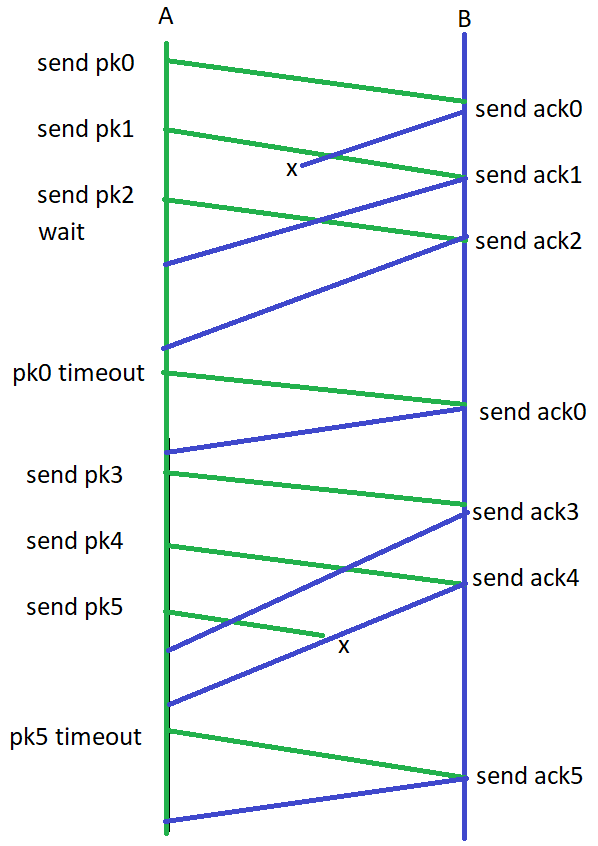
\includegraphics[width=300px]{assets/GBN.png}
				\caption{Illustration of GBN}
			\end{figure}
		\subsection{When will buffering improve performance for GBN}
			In the case of a large windows size, and the first package is lost but the rest is received, when the first package is then resent and aknowledgment equal to window size.
	\section{Lecture 5}
		\subsection{Flow control: A large file is being trasnfered from A (120Mbps) to B (50Mbps) via a link (100Mbps), describe the flow controle}
			The flow controle will establish a windows for the TCP packages, such the receiver B will not overflow the reading buffer.
		\subsection{Duplicate acks: Why wait for three duplicate acks and not just at the first dublicate}
			Three is choosen since a double could accour in the event of out of order, but three will most likely be a missing segment.
		\subsection{Flow+Conguestion control: In the scenario where the receiver buffer is large enough for a full file and the A can send with 10 times link speed what is the limiting factor}
			The limit will be by the link and the congeustion controle. When A tries to send more than the link speed there will be dropped packages and therefore limit the amount of data sent.\\
			According to the choosen conguestion controle mechanism, it will be zig-zag around the limit of sending speed.
		\subsection{Comparing GBN, SR, TCP: In the scenario with 5 data segments send at once from A to B and 2nd segment is lost}
			\subsubsection{How many segments, acks have benn sent and what are their sequence numbers}
				\begin{itemize}
					\item GBN 9 segm \& 8 ack - seg1, seg2, seg3, seg4, seg5, ack2, nack3, nack4, nack5, seg2, seg3, seg4, seg5, ack3, ack4, ack5, ack6
					\item SR 6 segm \& 6 ack - seg1, seg2, seg3, seg4, seg5, ack2, ack2, ack2, ack2, seg2, ack6
					\item TCP: both option for GBN and SR are possible dependent on the implementation
				\end{itemize}
			\subsubsection{If the timeout value is larger than 5RTT which method is fastest}
				\begin{enumerate}
					\item TCP - using fast retransmit and receiver buffer
					\item GBN
					\item SR - since it has to wait 5RTT where GBN will know before that somethign went wrong
				\end{enumerate}
		\subsection{Large files and seequence numbers: Consider the transfer of file size $L$ bytes and an MSS of 536 bytes}
			\subsubsection{What is the maximum size of $L$ such the sequnce number is not exhausted}
				When sending the segment number will be for the next expected byte. Therefore the maximum number can be divided by the MSS.\\
				The maximum segment number is $2^{32}$.\\
				Therefore the maximum size of the file is $2^{32}/536=8.01\cdot 10^6$
			\subsubsection{How long would it take to send, with an extra 66 bytes of data over a 155 Mbps link. Assume no flow control and congestion control}
				$\frac{(536+66)\text{byte}\cdot 8.01\cdot 10^6}{155\text{Mbps}}=248.97\text{s}$
		\subsection{End-point auth}
			\subsubsection{Are an UDP request able to spoof en ip in the header and receive the answer}
				The answer will be sent to the spoofed ip address by. This therefore make UDP somewhat vulnerable since it can be used for DoS attacks agains the spoofed ip or if the UDP results in a change on the server which is only permitted by some ip's
			\subsubsection{After a server receive a synACK with correct sequence number can it be sure that the TCP request is not spoofed in case of a non man-in-the-middle attack}
				This would only happend if the attacker could predict the sequence number and therefore be able to sent first an initiater, predict the sequence number and send it back in synACK.\\
				This is therefore very unlikely if not impossible in correct implementations.
	\section{Lecture 6}
		\subsection{Diffie-Hellman}
			\subsubsection{Prove that in general Alice and Bob obtain the same symmetric key that is prive $S=S'$}
				\begin{align*}
					T_A=g^{S_A}\mod p\\
					T_B=g^{S_B}\mod p\\
					S=T_B^{S_A}\mod p\\
					S'=T_A^{S_B}\mod p\\
					S=(g^{S_A}\mod p)^{S_B}\mod p\\
					S=g^{S_AS_B}\mod p\\
					S'=(g^{S_A}\mod p)^{S_B}\mod p\\
					S'=g^{S_BS_A}\mod p\\
					S'=S
				\end{align*}
			\subsubsection{With $p=11$ and $g=2$ suppose Alice and Bob choose private keys $S_A=5$ and $S_B=12$ respectively. Calculate Alice's and Bob's public keys $T_A$ nad $T_B$}
				\begin{align*}
					T_A=g^{S_A}\mod p\\
					T_A=2^5\mod 11
					T_A=10
					T_B=g^{S_B}\mod p\\
					T_B=2^{12}\mod 11\\
					T_B=4
				\end{align*}
			\subsubsection{Following up on part b now calculate $S$ as the shared symmetric key}
				\begin{align*}
					S=g^{S_AS_B}\mod p\\
					S=2^60\mod 11\\
					S=1
				\end{align*}
			\subsubsection{Provide a timeing diagram that show how Diffie-Hellman can be attacked by a man-in-the-middle. The timing diagram should have three vertical lines, one for Alice, one for Bob, and one for the attacker Trudy, Discuss also how this can be avoided.}
				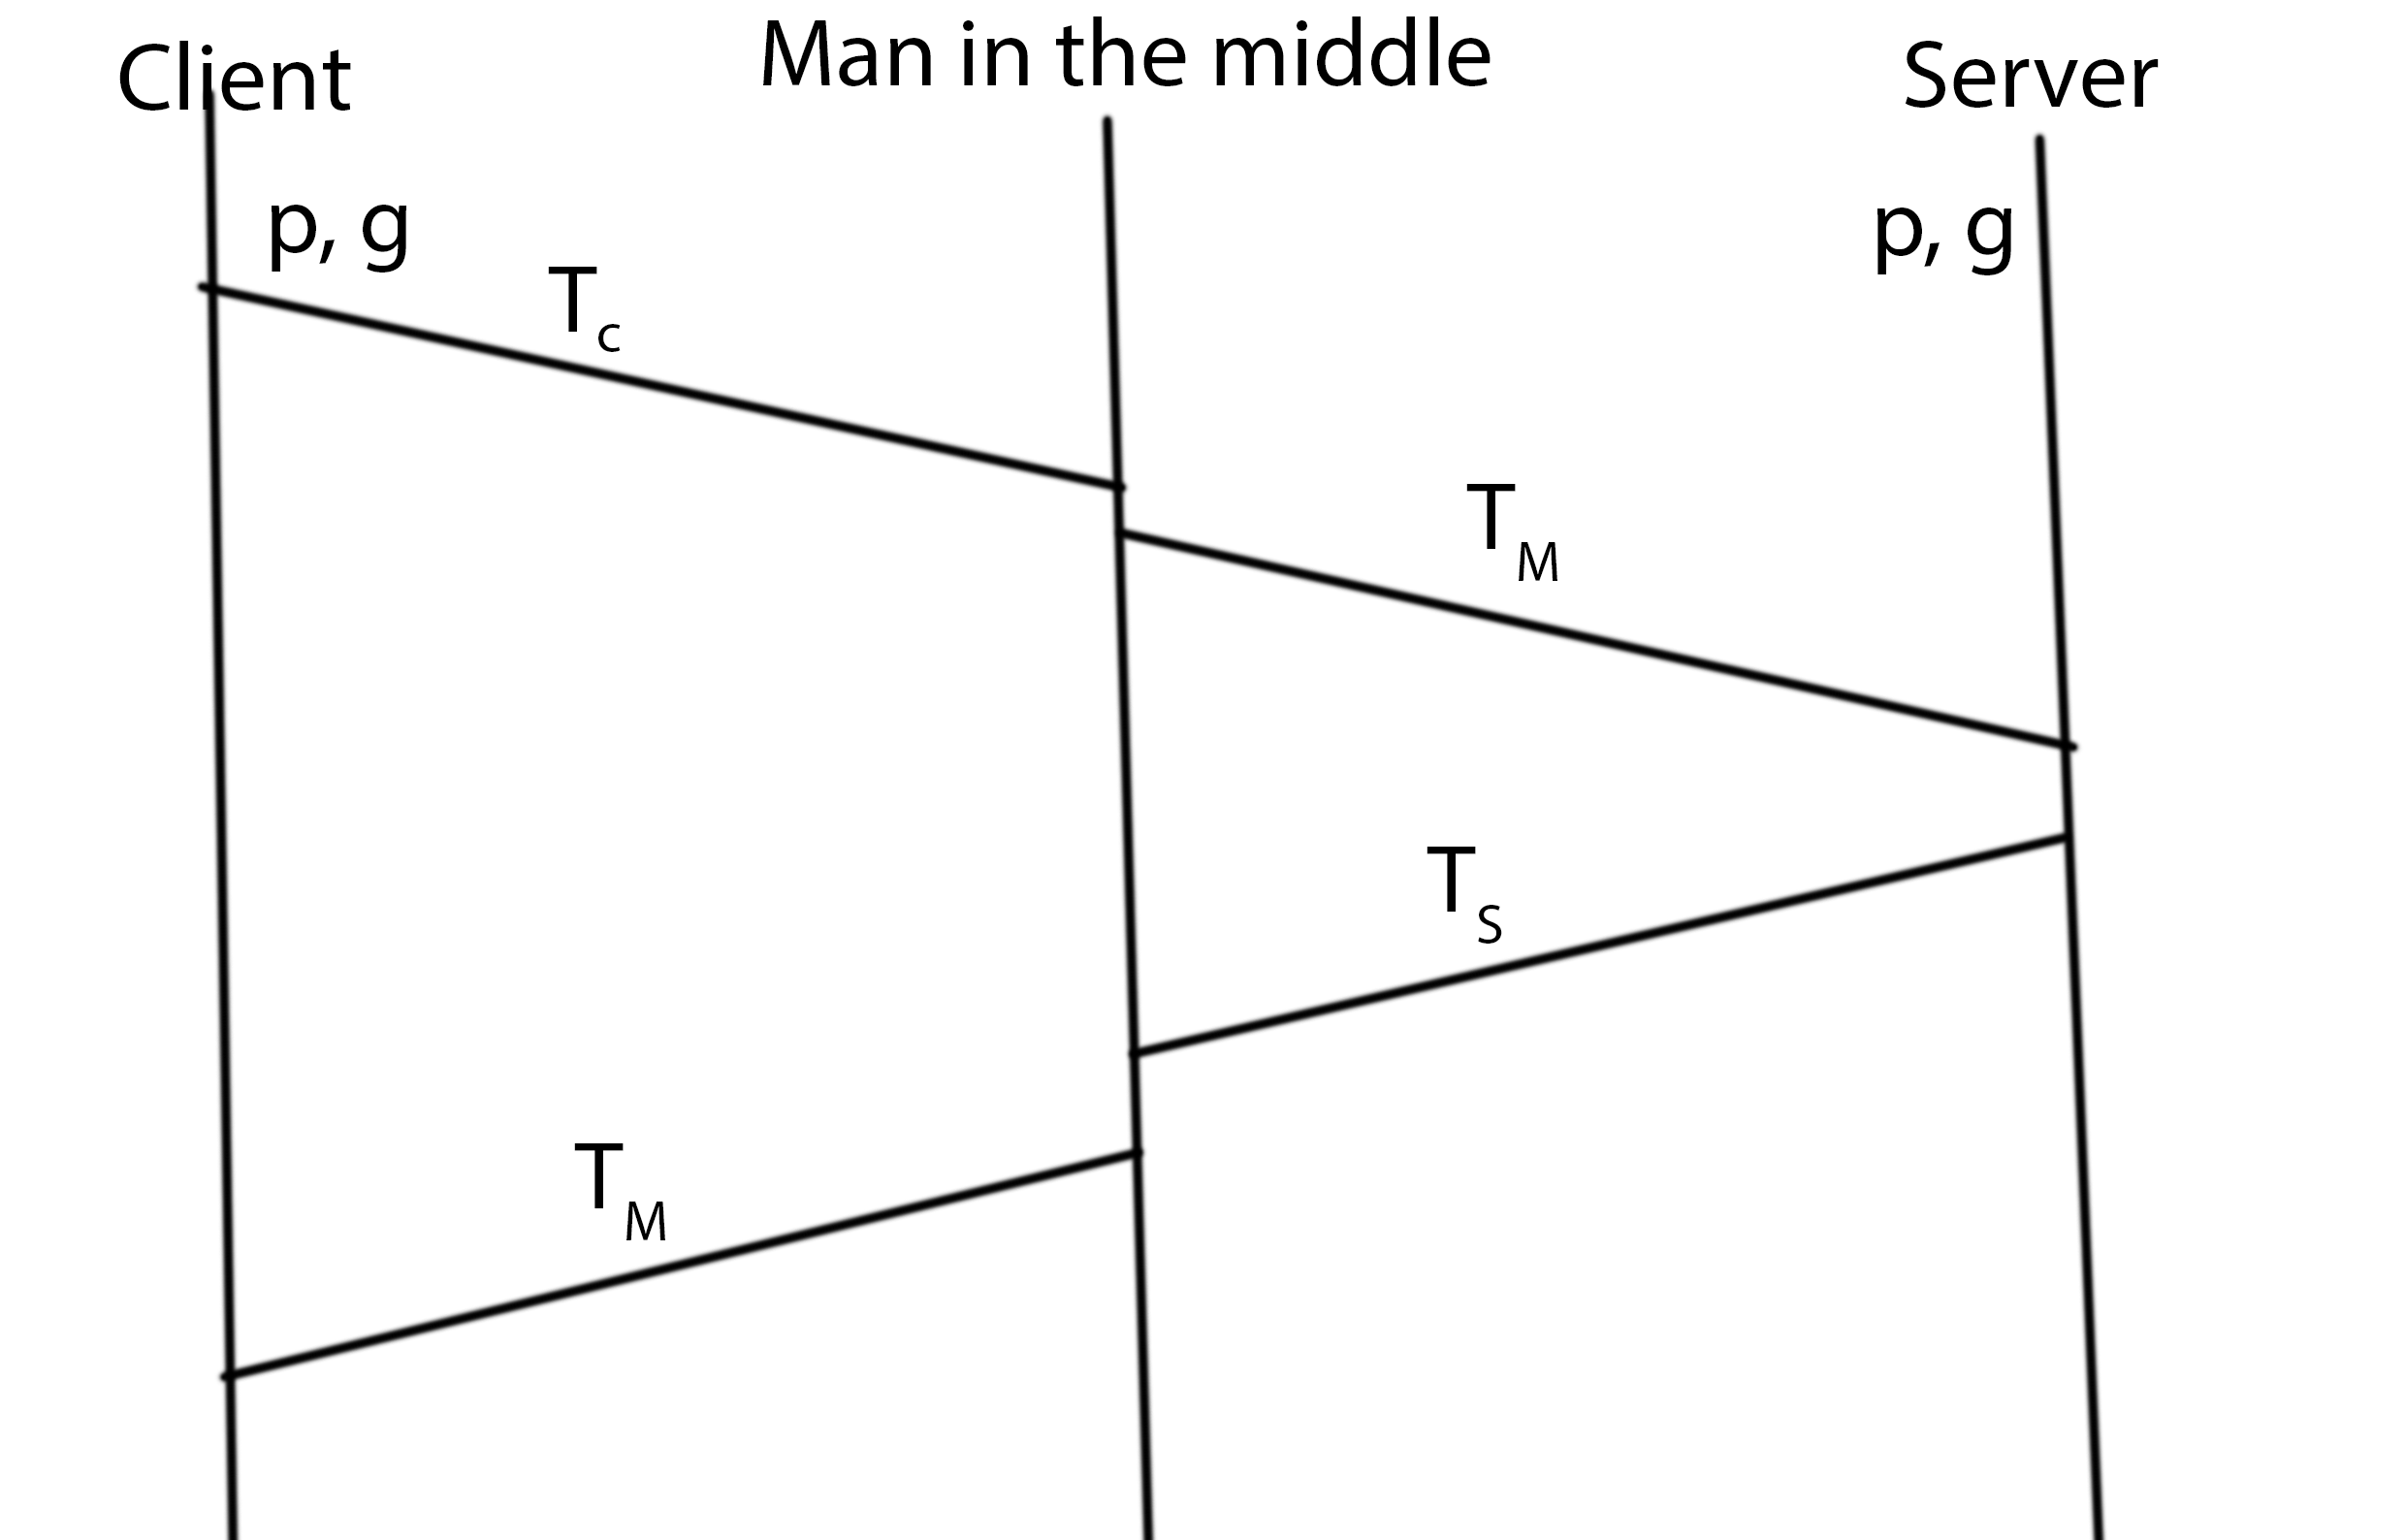
\includegraphics[width=300px]{assets/DiffieHellman.png}
		\subsection{Wireshark and SSL}
			\subsubsection{Is Wireshark packet 112 sent by the client or server}
				Client
			\subsubsection{What is the servers IP address and port number}
				216.75.194.220\\
				2271
			\subsubsection{Assuming no loss and no retransmissions what will be the sequence number of the next TCP segment sent by the client}
				Current 79\\
				Len: 204\\
				next 283
			\subsubsection{How many SSL record does wireshark packet 112 contain}
				3
			\subsubsection{Assumng that the handshake type field is 1 byte and each length field is 3 bytes, what are the values of the first and last bytes of the Master Secret (or Encrypted Master Secret)}
				Start with 00 and end with 29
		\subsection{Will SSL at the receiving side accept the bogus packet and pass the payload tothe receiving application? Why or why not}
			No since the sequence is part of the hash, will the hash not match and the packet will be thrown away.
	\setcounter{section}{7}
	\section{Lecture 8}
		\subsection{Consider the network below}
			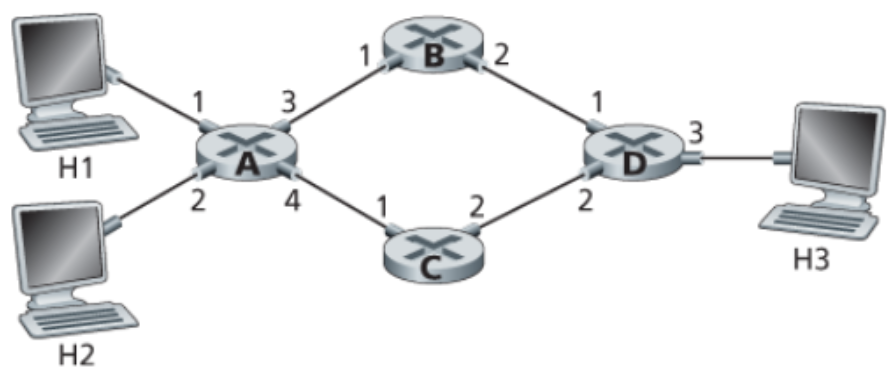
\includegraphics[width=300px]{assets/7.1.png}
			\subsubsection{Show the forwarding table in router A, such that all traffix destined to host 3 us forwarded using interface 3}
				H3 IP prefix - 3\\
			\subsubsection{Write a forwarding table such that all traffic from H1 destined to host H3 is forwarded through interface 3, while all traffic from H2 destined to host H3 is forwarded through interface 4}
				This is not possible with a forwarding table since it would be router A which should forward the two different package but since the senders ip is not included in the table can the packages not be distringuished.
		\subsection{Longest prefix matching and number of addresses}
			Consider a datagram network using 8-bit host addresses. Suppose a router uses longest prefix matching and has the following forwarding table\\
			11 - 0\\
			101 - 1\\
			100 - 2\\
			otherwise - 3\\
			For each of the four interfaces, give the associated range of destination host addresses and the number of addresses in the range\\
			Since the prefix for 0 is 11 the range will be $2^{8-2}=2^6$\\
			For the other is will be $2^{8-3}=2^5$
		\subsection{CIDR notation}
			Consider a router that interconnects three subnets: Subnet 1, Subnet 2, and Subnet 3. Suppose all of the interfaces in each of these three subnets are required to have the prefix 223.1.17/24. Also suppose that Subnet 1 is required to support at least 62 interfaces, Subnet 2 is to support at least 106 interfaces, and Subnet 3 is to support at least 15 interfaces. Provide three network addresses (of the form a.b.c.d/x) that satisfy these constraints.\\
			62 $< 2^6$\\
			106 $< 2^7$\\
			15 $< 2^4$\\
			subnet 1 - 223.1.17.4/6\\
			subnet 2 - 223.1.17.1/7\\
			subnet 3 - 223.1.17.20/4
		\subsection{Nat translation table}
			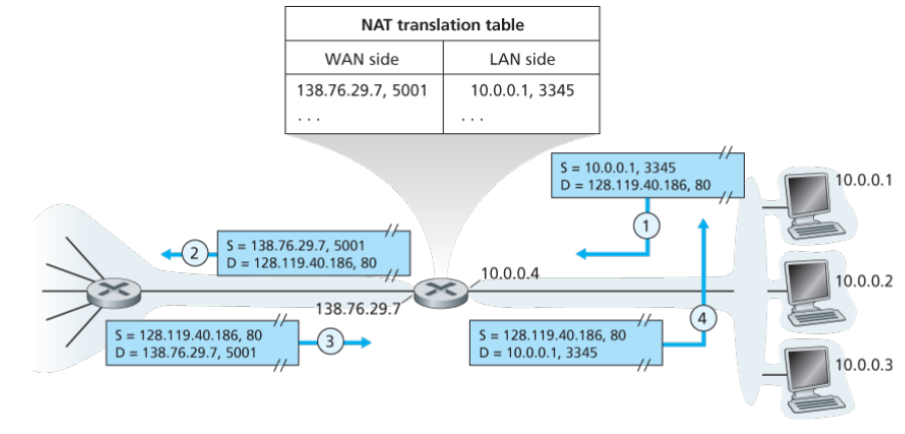
\includegraphics[width=300px]{assets/7.4.png}\\
			Suppose that the ISP instead assigns the router the address 24.34.112.235 and that the network address of the home network is 192.168.1/24. .. Assign addresses to all interfaces in the home network. .. Suppose each host has two ongoing TCP connections, all to port 80 at host 128.119.40.86. Provide the six corresponding entries in the NAT translation table.\\
			192.168.1.1\\
			192.168.1.2\\
			192.168.1.3\\
			Table entries\\
			128.119.40.86, 80 | 192.168.1.1 , 1234\\
			128.119.40.86, 80 | 192.168.1.2, 1234\\
			128.119.40.86, 80 | 192.168.1.3, 1234
		\subsection{MTU and fragmentation}
			Consider sending a 1600-byte datagram into a link that has an MTU of 500 bytes. Suppose the original datagram is stamped with the identification number 291. How many fragments are generated? What are the values in the various fields in the IP datagram(s) generated related to fragmentation?\\
			This will be in 4 fragments, since even accounting for header sizes of 20 bytes.
		\subsection{Nat and P2P}
			What is the problem of NAT in P2P applications? How can it be avoided? Is there a special name for this solution\\
			The problem is ingoing connection having to find the open address. The is done with a NAT tool which searches the local network for open connections
		\subsection{Switch fabric}
			Suppose two packets arrive to two different input ports of a router at exactly the same time. Also suppose there are no other packets anywhere in the router
			\subsubsection{Suppose the two packets are to be forwarded to two different output ports. Is it possible to forward the two packets through the switch fabric at the same time when the fabric uses a shared bus?}
				No the bus will only be able to handle one package at the time
			\subsubsection{What about switching via memory}
				In case of a multi core processor this would be possible
			\subsubsection{What about crossbar}
				In a crossbar they will be able to pass through to output at the same time.
	\section{Lecture 9}
		\subsection{BGP and AS-Path}
			Will a BGP router always choose the loop-free route with the shortest ASpath length? Justify your answer.\\
			A loop-free route will always be choosen in case of non negative weights. In this case it would never be desireable to make a loop.\\
			A negative weight could happen in case of admin choosen weight.
		\subsection{Routing protocols}
			Consider the network.\\
			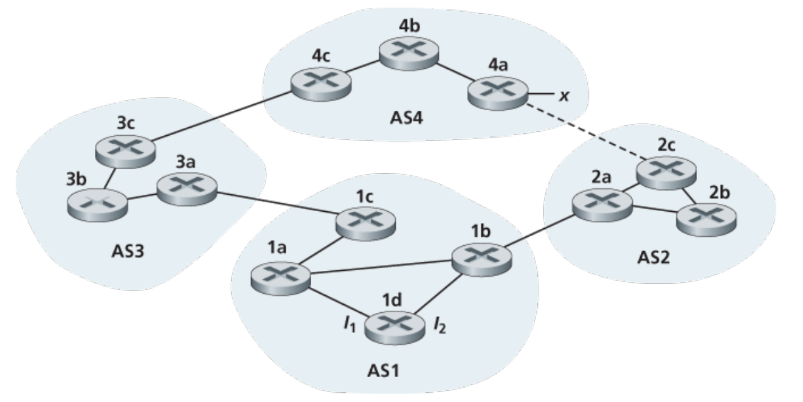
\includegraphics[width=300px]{assets/9.2.png}\\
			Suppose AS3 and AS2 are running OSPF for their intra-AS routing protocol.\\
			Suppose AS1 and AS4 are running RIP for their intra-AS routing protocol.\\
			Suppose eBGP and iBGP are used for the inter-AS routing protocol.\\
			Initially suppose there is no physical link between AS2 and AS4
			\subsubsection{Router 3c learns about prefix x from which routing protocol: OSPF, RIP, eBGP, or iBGP}
				It will learn it from eBGP
			\subsubsection{Router 3a learns about x from which routing protocol}
				iBGP
			\subsubsection{Router 1c learns about x from which routing protocol}
				eBGP
		\subsection{BGP and routing traffic}
			Suppose ASs X and Z are not directly connected but instead are connected by AS Y. Further suppose that X has a peering agreement with Y, and that Y has a peering agreement with Z. Finally, suppose that Z wants to transit all of Y’s traffic but does not want to transit X’s traffic. Does BGP allow Z to implement this policy?\\
			Yes if using the route selection aglorithm.
		\subsection{Poisoned reverse and count-to-infinity problem}
			Can the poisoned reverse solve the general count-to-infinity problem?
			No in the system\\
			A - C - D\\
			\;\textbackslash\;\; / \\
			. B\\
			And the shortest path from B to D is B A C D\\
			C D then breaks, this will poison C to A but when C then searched for new D it will find it via B and then create a couting loop.
		\subsection{BGP and ISP peering}
			Consider the following network\\
			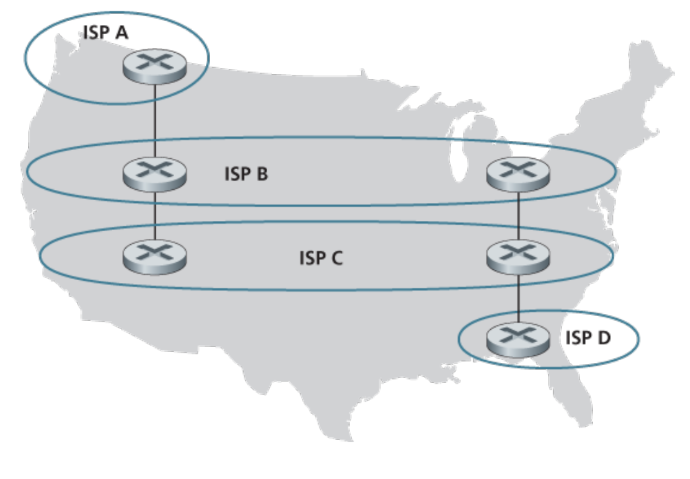
\includegraphics[width=300px]{assets/9.5.png}\\
			By using local\_pref the bgp can force isp B to handover data on given gateways on the east coast.
			
\end{document}
